%\adparagraph{Rating nDCG}

\begin{figure}[H]
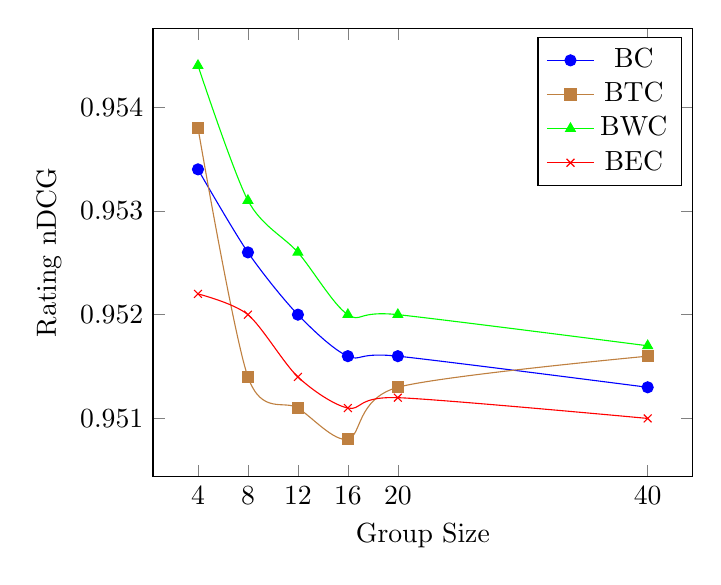
\begin{tikzpicture}
\begin{axis}[
	y tick label style={
        /pgf/number format/.cd,
            fixed,
            fixed zerofill,
            precision=3,
        /tikz/.cd
    },
	xlabel=Group Size,
	ylabel=Rating nDCG,
	xtick = {4,8,12,16,20,40}]
	\addplot[smooth,mark=*,blue] plot coordinates {
		(4,0.9534)
		(8,0.9526)
		(12,0.952)
		(16,0.9516)
		(20,0.9516)
		(40,0.9513)
	};
	\addlegendentry{BC}
	
	\addplot[smooth,color=brown,mark=square*] plot coordinates {
		(4,0.9538)
		(8,0.9514)
		(12,0.9511)
		(16,0.9508)
		(20,0.9513)
		(40,0.9516)
	};
	\addlegendentry{BTC}
	
	
	\addplot[smooth,color=green,mark=triangle*] plot coordinates {
		(4,0.9544)
		(8,0.9531)
		(12,0.9526)
		(16,0.952)
		(20,0.952)
		(40,0.9517)
	};
	\addlegendentry{BWC}
	
	
	\addplot[smooth,color=red,mark=x] plot coordinates {
		(4,0.9522)
		(8,0.9520)
		(12,0.9514)
		(16,0.9511)
		(20,0.9512)
		(40,0.951)
	};
	\addlegendentry{BEC}

\end{axis}
\end{tikzpicture}
\caption{Results using Rating nDCG on BC extensions}\label{fig:appenixrndcg}
\end{figure}